% Diapositiva 15

% Luchando los dias

%============================================
% 13. cómo se usaron dentro de la simulación la formula de las amplitudes ideales.
% 14. Explicar el valor usado para A0
%=============================================

\begin{frame}{Generación de Amplitudes Simuladas}

    \begin{columns}[T] % Alineación superior para evitar desplazamientos
        
        %========================================
        % COLUMNA IZQUIERDA: VISUALIZACIÓN
        %========================================
        \column{0.55\textwidth}
        \begin{center}
            % Reducimos un poco la imagen para ganar espacio vertical
            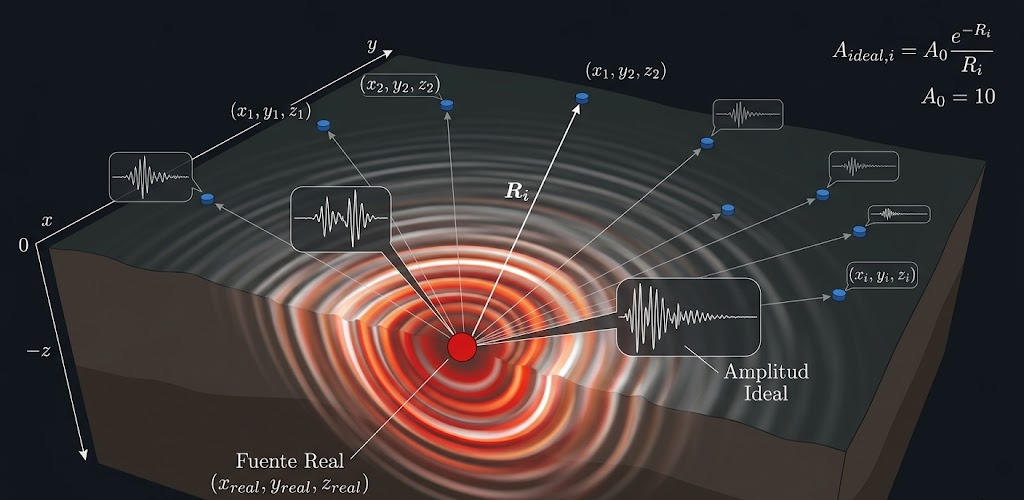
\includegraphics[width=0.85\textwidth]{Imagenes/Amplitudes_Ideales.png}
            
            \vspace{0.1cm}
            \tiny \textcolor{gray}{
                Distribución de sensores y fuente sísmica simulada.
            }
        \end{center}

        %========================================
        % COLUMNA DERECHA: MODELO Y SÍNTESIS
        %========================================
        \column{0.42\textwidth}
        
        \begin{block}{Modelo de Simulación}
            \centering
            \small
            $A_0 = 10$
            \vspace{0.1cm}
            \[
            A_{ideal,i} = A_0 \frac{e^{-R_i}}{R_i}
            \]
        \end{block}

        \vspace{0.2cm} % Espacio reducido entre bloques

        \begin{block}{Flujo de Información}
            \scriptsize
            \begin{itemize}
                \item \textbf{Cálculo:} Amplitudes obtenidas mediante distancias $R_i$.
                \item \textbf{Transición:} Datos de entrada para el problema inverso.
            \end{itemize}
        \end{block}

    \end{columns}

    \vspace{0.3cm} % Espacio controlado para la frase final

    \begin{center}
        \footnotesize
        \textbf{El modelo directo construye el escenario que el algoritmo inverso deberá resolver.}
    \end{center}

\end{frame}
